\section{Experiments}\label{exp}
\subsection{Benchmark and Evaluation}
We evaluate our method and baselines on \textbf{KernelBench}~\citep{ouyang2025kernelbenchllmswriteefficient}, a popular benchmark designed to assess the ability of LLMs to generate CUDA kernels.  
KernelBench consists of multiple difficulty levels, and we adopt all tasks from Level 1 to Level 3, resulting in a total of 250 tasks.  
Specifically, Level 1 contains relatively simple 100 tasks involving basic operators (e.g., matrix multiplication),  
Level 2 includes medium-difficulty 100 tasks composed of multi-step operator combinations,  
and Level 3 contains 50 challenging tasks involving full neural network architectures (e.g., AlexNet).  
Each task is accompanied by a reference PyTorch implementation and predefined input/output specifications, which enables fully automated and reliable evaluation of both correctness and performance. Details of KernelBench are provided in Appendix~\ref{KernelBench}. 

Due to the high computational cost of running experiments for some ablation studies, we do not evaluate them on the entire KernelBench benchmark. 
Instead, we construct a {stratified random subset} of tasks, denoted as $\mathcal{D}^{*}$, by sampling proportionally from each difficulty level of KernelBench. This ensures that $\mathcal{D}^{*}$ maintains the same task distribution as the full benchmark while enabling fair and efficient evaluation. Specifically, $\mathcal{D}^{*}$ contains a total of 25 tasks, with 10 tasks in Level 1, 10 tasks in Level 2 and 5 tasks in Level 3. More details on the construction of $\mathcal{D}^{*}$ are provided in Appendix~\ref{subset}.


We evaluate model performance on KernelBench using the following metrics: (1) \textbf{Correctness}: the fraction of tasks for which the generated kernel compiles successfully and produces outputs identical to the PyTorch reference on all test cases. (2) \textbf{Performance}: the ratio of the execution speed (tested on a specific GPU), between a correct generated kernel and its PyTorch reference. 
(3) \textbf{Fast\(_1\)} : the proportion of correct kernels whose execution speed exceeds their PyTorch reference. 
(4) \textbf{Median speedup}: the median of `Performance' values across all tasks, reflecting typical rather than average behavior.
(5) \textbf{75th percentile speedup}: the 75th percentile of Performance values, capturing upper-quartile efficiency.


For methods that perform iterative refinement or generate multiple candidates (including \agentname), we report the best-performing correct kernel among all candidates for each task.


\subsection{Settings \& Baselines}
In our main results, we instantiate \agentname~with OpenAI-o3 as both the Coder and the Judge as our {\it default} setting.  
We set the maximum number of iteration rounds to $N{=}10$ to balance performance improvements and inference cost.  
Unless otherwise stated, all methods are evaluated under the same compilation/runtime environment in Quadro RTX 6000 and task-specific test suites. 

To contextualize the performance of \agentname~and assess the effect of advanced foundation models, we include the following baselines for the main results and ablation studies:

\begin{itemize}

    \item OpenAI-o3: Using OpenAI-o3 for one-shot generation without iteration;  
    \item o3-self-refine(our baseline): Using OpenAI-o3 for ten rounds of self-refinement without a Judge, where the model relies solely on itself to correct and optimize kernels given hardware feedback;  
    \item o3-correction(our baseline): A variant of \agentname~where the Judge provides only correctness feedback but no optimization feedback;  
    \item o3-optimization(our baseline): A variant of \agentname~where the Judge provides only optimization feedback but no correction feedback;  
    \item Kevin-32B: a strong RL-based model for CUDA kernel optimization from \citep{kevin-multi-turn-rl}. We directly take results from their official paper.  
    % \item Kevin-H200: Kevin-32B in H200, we directly use results reported in ~\citep{kevin-multi-turn-rl}.
    \item Agentic Baseline: the agentic workflow from \citep{lange2025robustagenticcudakernel}, a strong multi-agent baseline, which uses an LLM ensemble including both
reasoning (o3 \& o4-mini) and conventional LLMs (Claude Sonnet 3.7 \& GPT-4.1).
    \item \agentname~(full metrics): a variant of \agentname~where the Judge leverages the entire set of NCU metrics.
\end{itemize}


This baseline setting enables a comprehensive comparison across (i) base model vs.\ corresponding agent-based method, (ii) the presence/absence of Judge feedback, (iii) RL-based vs.\ training-free agent-based approaches, and (iv) different agentic methods. 

\begin{table}[t]
\caption{Main results on KernelBench (Level 1-3, 250 tasks). Results of Agentic Baseline is on Level 1 and 2. All experiments here are run in RTX 6000. Methods evaluated on \(\mathcal{D}^{*}\) are marked with \(^*\). \agentname-Scaling Up means scaling up maximum iteration rounds}

\label{tab:main_results}
\centering
\begin{tabular}{lcccccc}
\toprule
\textbf{Method} & \textbf{Correct$\uparrow$} & \textbf{Median $\uparrow$}  & \textbf{75\% $\uparrow$}  & \textbf{Perf $\uparrow$}  & \textbf{Fast$_1$$\uparrow$} \\
\midrule
OpenAI-o3         & 57.6\% & 0.390 & 1.014 & 0.680  & 31.60\% \\
o3-self-refine        & 90.8\% & 1.012 & 1.209 & 1.107  & 55.20\% \\
o3-correction      & 97.6\% & 1.031 & 1.238 & 1.222  & 59.60\% \\
o3-optimization      & 88.4\% & 1.061 & 1.483 & 1.509  & 64.00\% \\
Agentic Baseline(Level 1 \& 2) & 95.0\% & --- & ---  & 1.490 & --- \\
\agentname(full metrics)$^{*}$   & 100\% & 1.280 & 1.489  & 1.414 & 80.00\% \\
 
\midrule
\agentname  & \textbf{97.6\%} & \textbf{1.107} & \textbf{1.592} & \textbf{1.677}  & \textbf{70.80\%} \\

\agentname(Level 1 \& 2)  & \textbf{98.0\%} & \textbf{1.112} & \textbf{1.617} & \textbf{1.776}  & \textbf{71.50\%} \\

\agentname$^{*}$ & \textbf{100\%} &  \textbf{1.322} & \textbf{1.736} & \textbf{1.767} & \textbf{84.00\%} \\
\agentname-Scaling Up$^{*}$ & \textbf{100\%} &  \textbf{1.317} & \textbf{1.777} & \textbf{2.265} & \textbf{92.00\%} \\
\bottomrule
\end{tabular}
\end{table}






\begin{table}[t]
\caption{Main results on KernelBench (Level 1-3, 250 tasks) of \agentname~ in RTX 6000.}
\label{tab:Level1-3}
\centering
\begin{tabular}{lccccc}
\toprule
\textbf{Task} & \textbf{Correct$\uparrow$} & \textbf{Median $\uparrow$}  & \textbf{75\% $\uparrow$}  & \textbf{Perf $\uparrow$}  & \textbf{Fast$_1$$\uparrow$} \\
\midrule
Level 1   & 96\% &  1.044 & 1.751 & 1.448 & 54.0\% \\
Level 2  & 100\% & 1.124 & 1.427 & 2.104 & 89.0\% \\
Level 3  & 96\% & 1.081& 1.510 & 1.283 & 68.0\% \\
\bottomrule
\end{tabular}
% \vspace{-5pt}
\end{table}

\subsection{Main Results in RTX 6000}
\label{sec:MainResults}
Table~\ref{tab:main_results} reports the main results in KernelBench. {\agentname} consistently outperforms all baselines across all metrics, both in the entire Kernelbench and in the stratified subset \(\mathcal{D}^{*}\) .


{On KernelBench, \agentname~attains \textbf{97.6\%} correctness with an average performance of \textbf{1.677$\times$}, and \textbf{70.8\% Fast$_1$}, while achieving a median speedup of 1.107$\times$ with a 75th percentile speedup of 1.592$\times$. These results significantly improve over the base model OpenAI-o3 and other ablated variants, including o3-self-refine, o3-correction and o3-optimization.}

{On the reduced dataset \(\mathcal{D}^{*}\), \agentname~achieves 100\% correctness, a median speedup of 1.322$\times$, a 75th percentile speedup of 1.736$\times$, an average performance of 1.767$\times$, and 84.0\% Fast$_1$.  
This substantially surpasses \agentname(full metrics), which reaches only 1.280$\times$ median, 1.489$\times$ at the 75th percentile, 1.414$\times$ performance, and 80\% Fast$_1$. Moreover, after scaling up maximum iteration rounds, \agentname-Scaling Up achieves a stronger performance, with \textbf{2.265$\times$} speedup. We will further discuss ablation studies using  \(\mathcal{D}^{*}\) in Section \ref{ablation} and scaling up maximum iteration rounds in Section \ref{scalingN}.}

\begin{figure}[t]
    \centering
    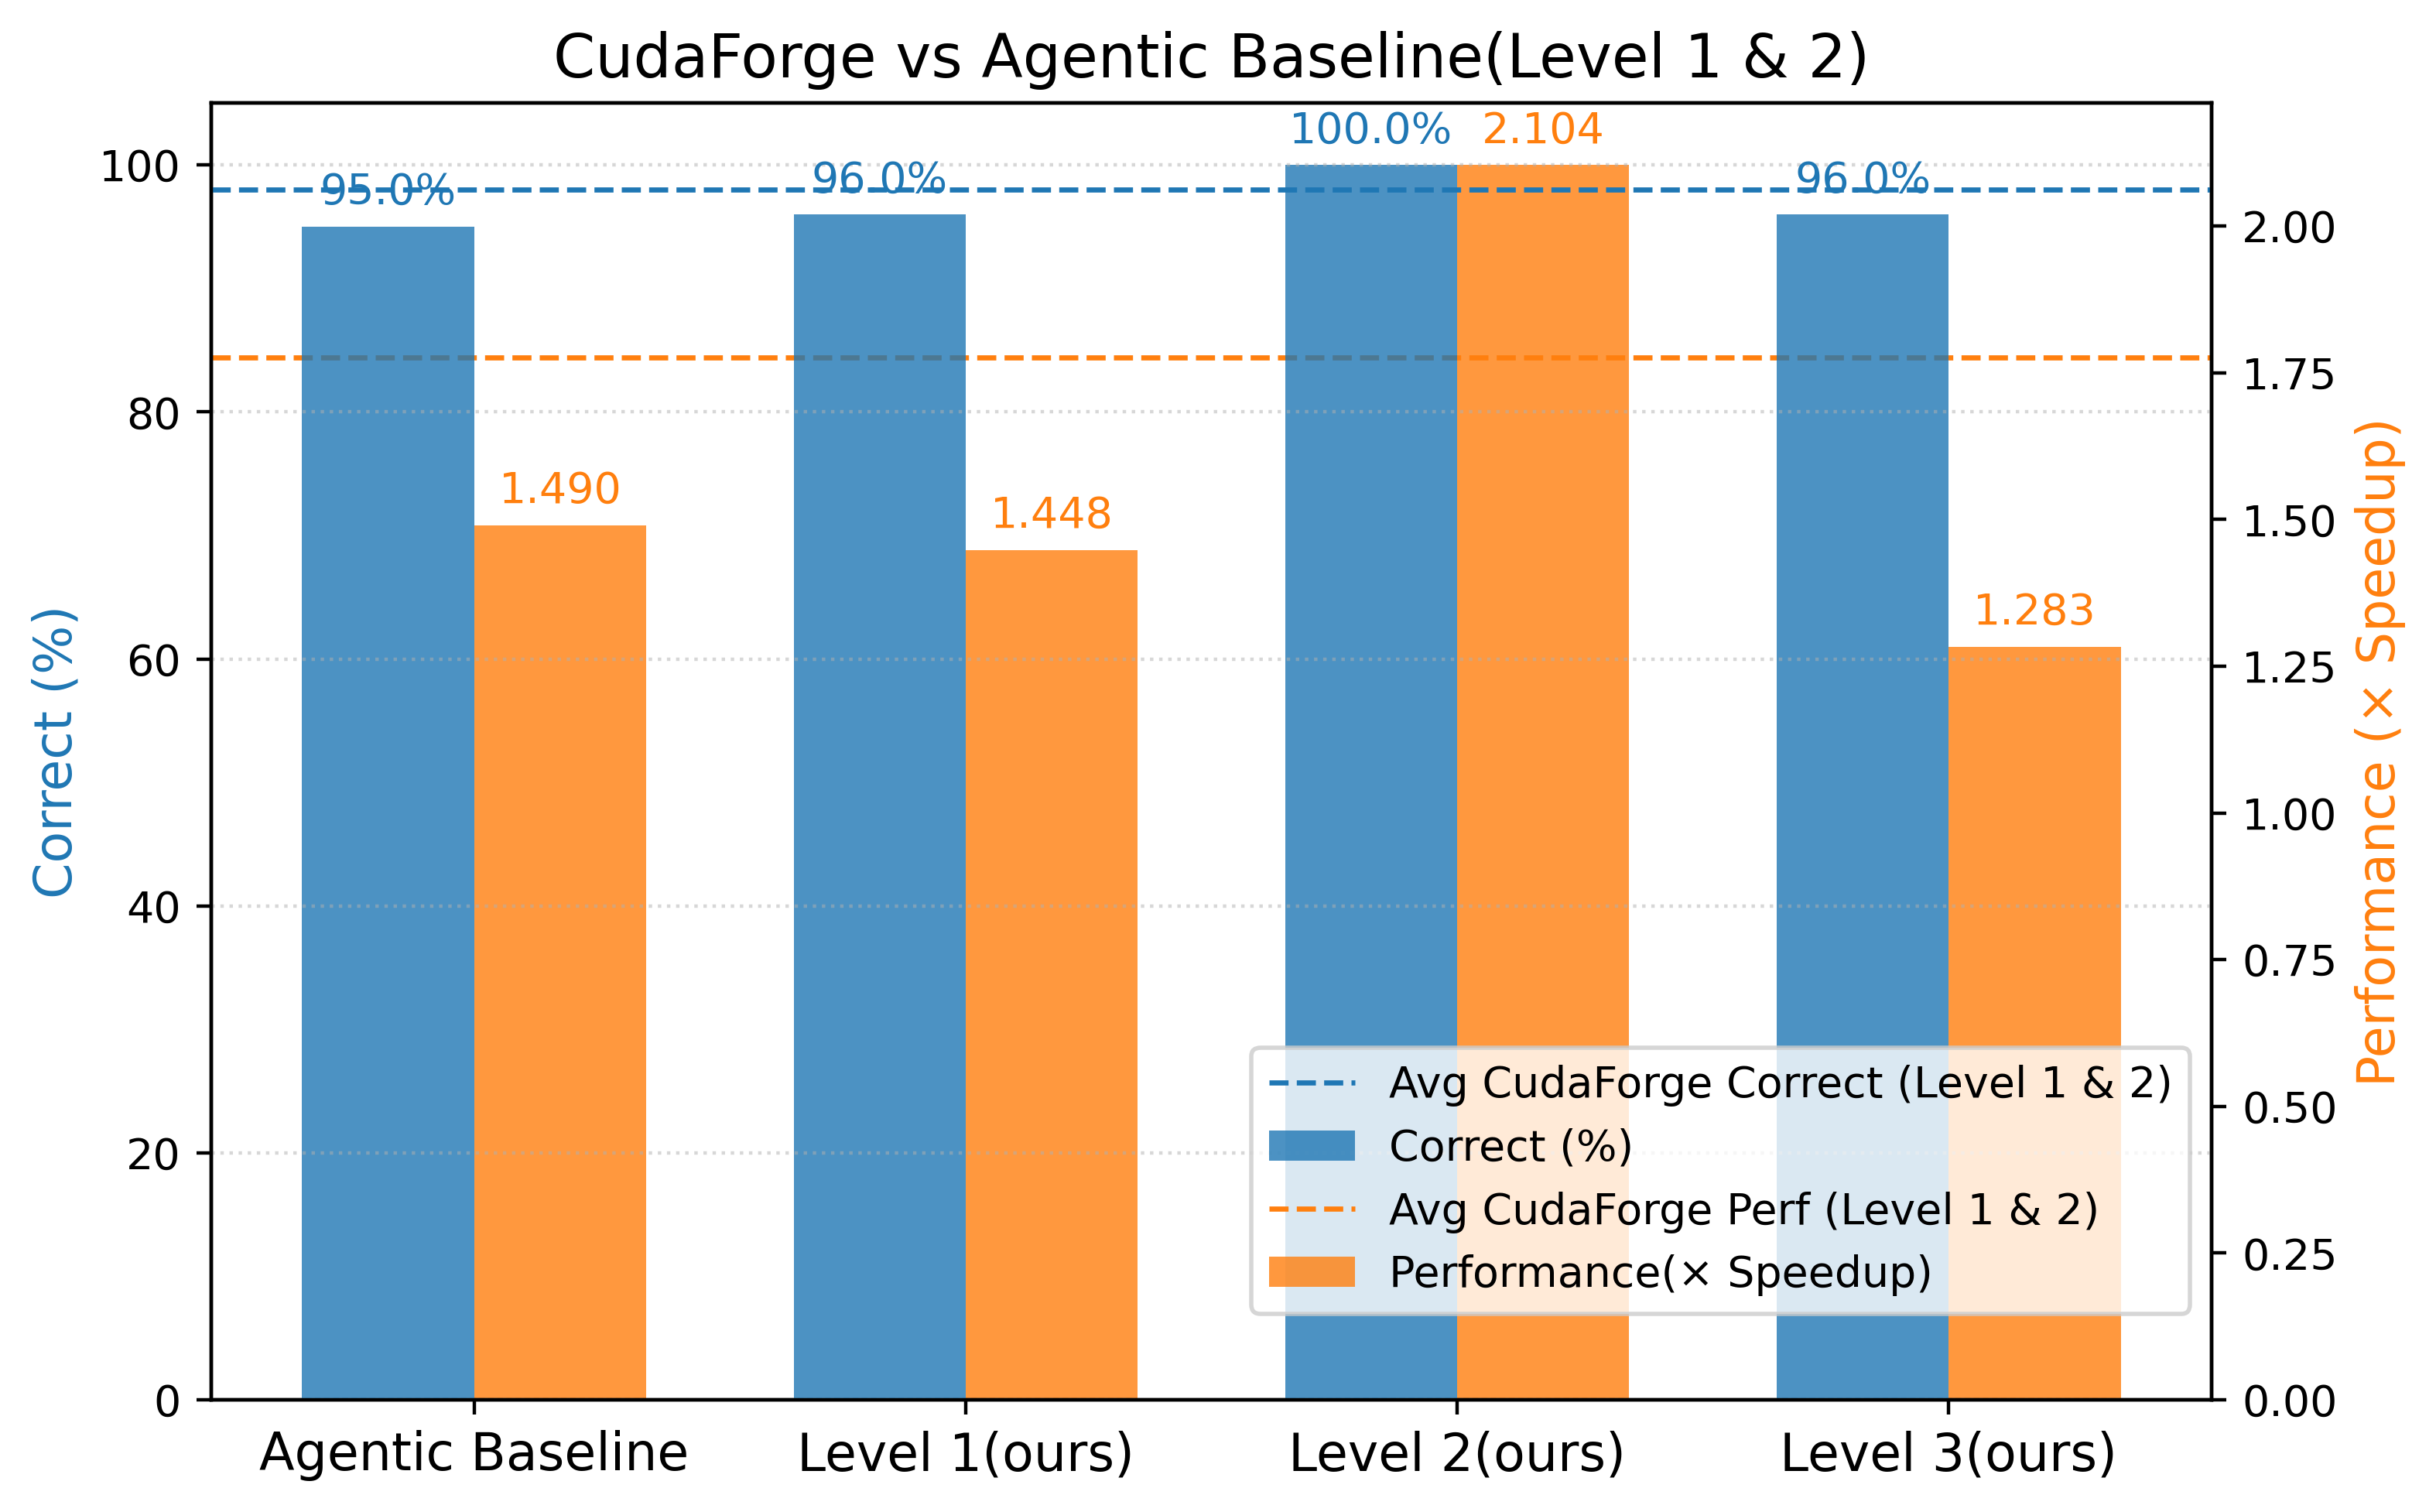
\includegraphics[width=0.85\linewidth]{pic/cuda_benchmark.png}
    \caption{
        Comparison of correctness and performance between \agentname~and the Agentic Baseline on KernelBench. Dashed lines denote average results of \agentname~over Level 1 and 2. \agentname~outperforms Agentic Baseline on KernelBench Level 1 and 2, and it also achieves strong performance in Level 3.
    }
    \label{fig:cuda_benchmark}
\end{figure}



We also compare \agentname~with Agentic Baseline\footnote{Note that it only reports results in Level 1 and 2, and we directly take the results from their paper since the paper has not open-sourced the code.} on KernelBench Level 1 and Level 2. As shown in Table~\ref{tab:main_results},~\ref{tab:Level1-3} and Fig~\ref{fig:cuda_benchmark}, \agentname ~achieves 98\% correctness and an average speedup of 1.776$\times$, which outperforms Agentic Baseline (95.0\%, 1.490$\times$), especially in speedup. This result shows our advantage compared to existing agentic work.

Notably, on Level 3, which represents the most challenging level of KernelBench, \agentname~achieves \textbf{96\%} correctness and an average \textbf{1.283$\times$} speedup.  
Given the complexity of Level 3 tasks, which involve full neural network architectures and multi-stage operations, these results demonstrate that \agentname~is capable of reliably generating and optimizing highly complex CUDA kernels, where prior approaches~\citep{kevin-multi-turn-rl,lange2025robustagenticcudakernel} have not explored it.

\subsection{{Comparison with Kevin-32B on H200}}
\label{Kevin}


In this subsection, we compare \agentname~with Kevin-32B~\citep{kevin-multi-turn-rl}. However, since Kevin-32B is not open-sourced—meaning that key details such as test-time prompts, evaluation setup, and benchmark specifications are not publicly available—a fully fair and reproducible comparison cannot be conducted.
According to the original paper, Kevin-32B was trained and evaluated on H200 GPUs using a self-constructed benchmark of comparable difficulty to KernelBench Levels 1 and 2. To ensure the comparison is as fair as possible under these constraints, we re-evaluate \agentname~on the same H200 hardware across KernelBench Levels 1–3,  aligning as much as possible our computational environment and evaluation protocol with those reported for Kevin-32B. 

\begin{figure}[t]
    \centering
    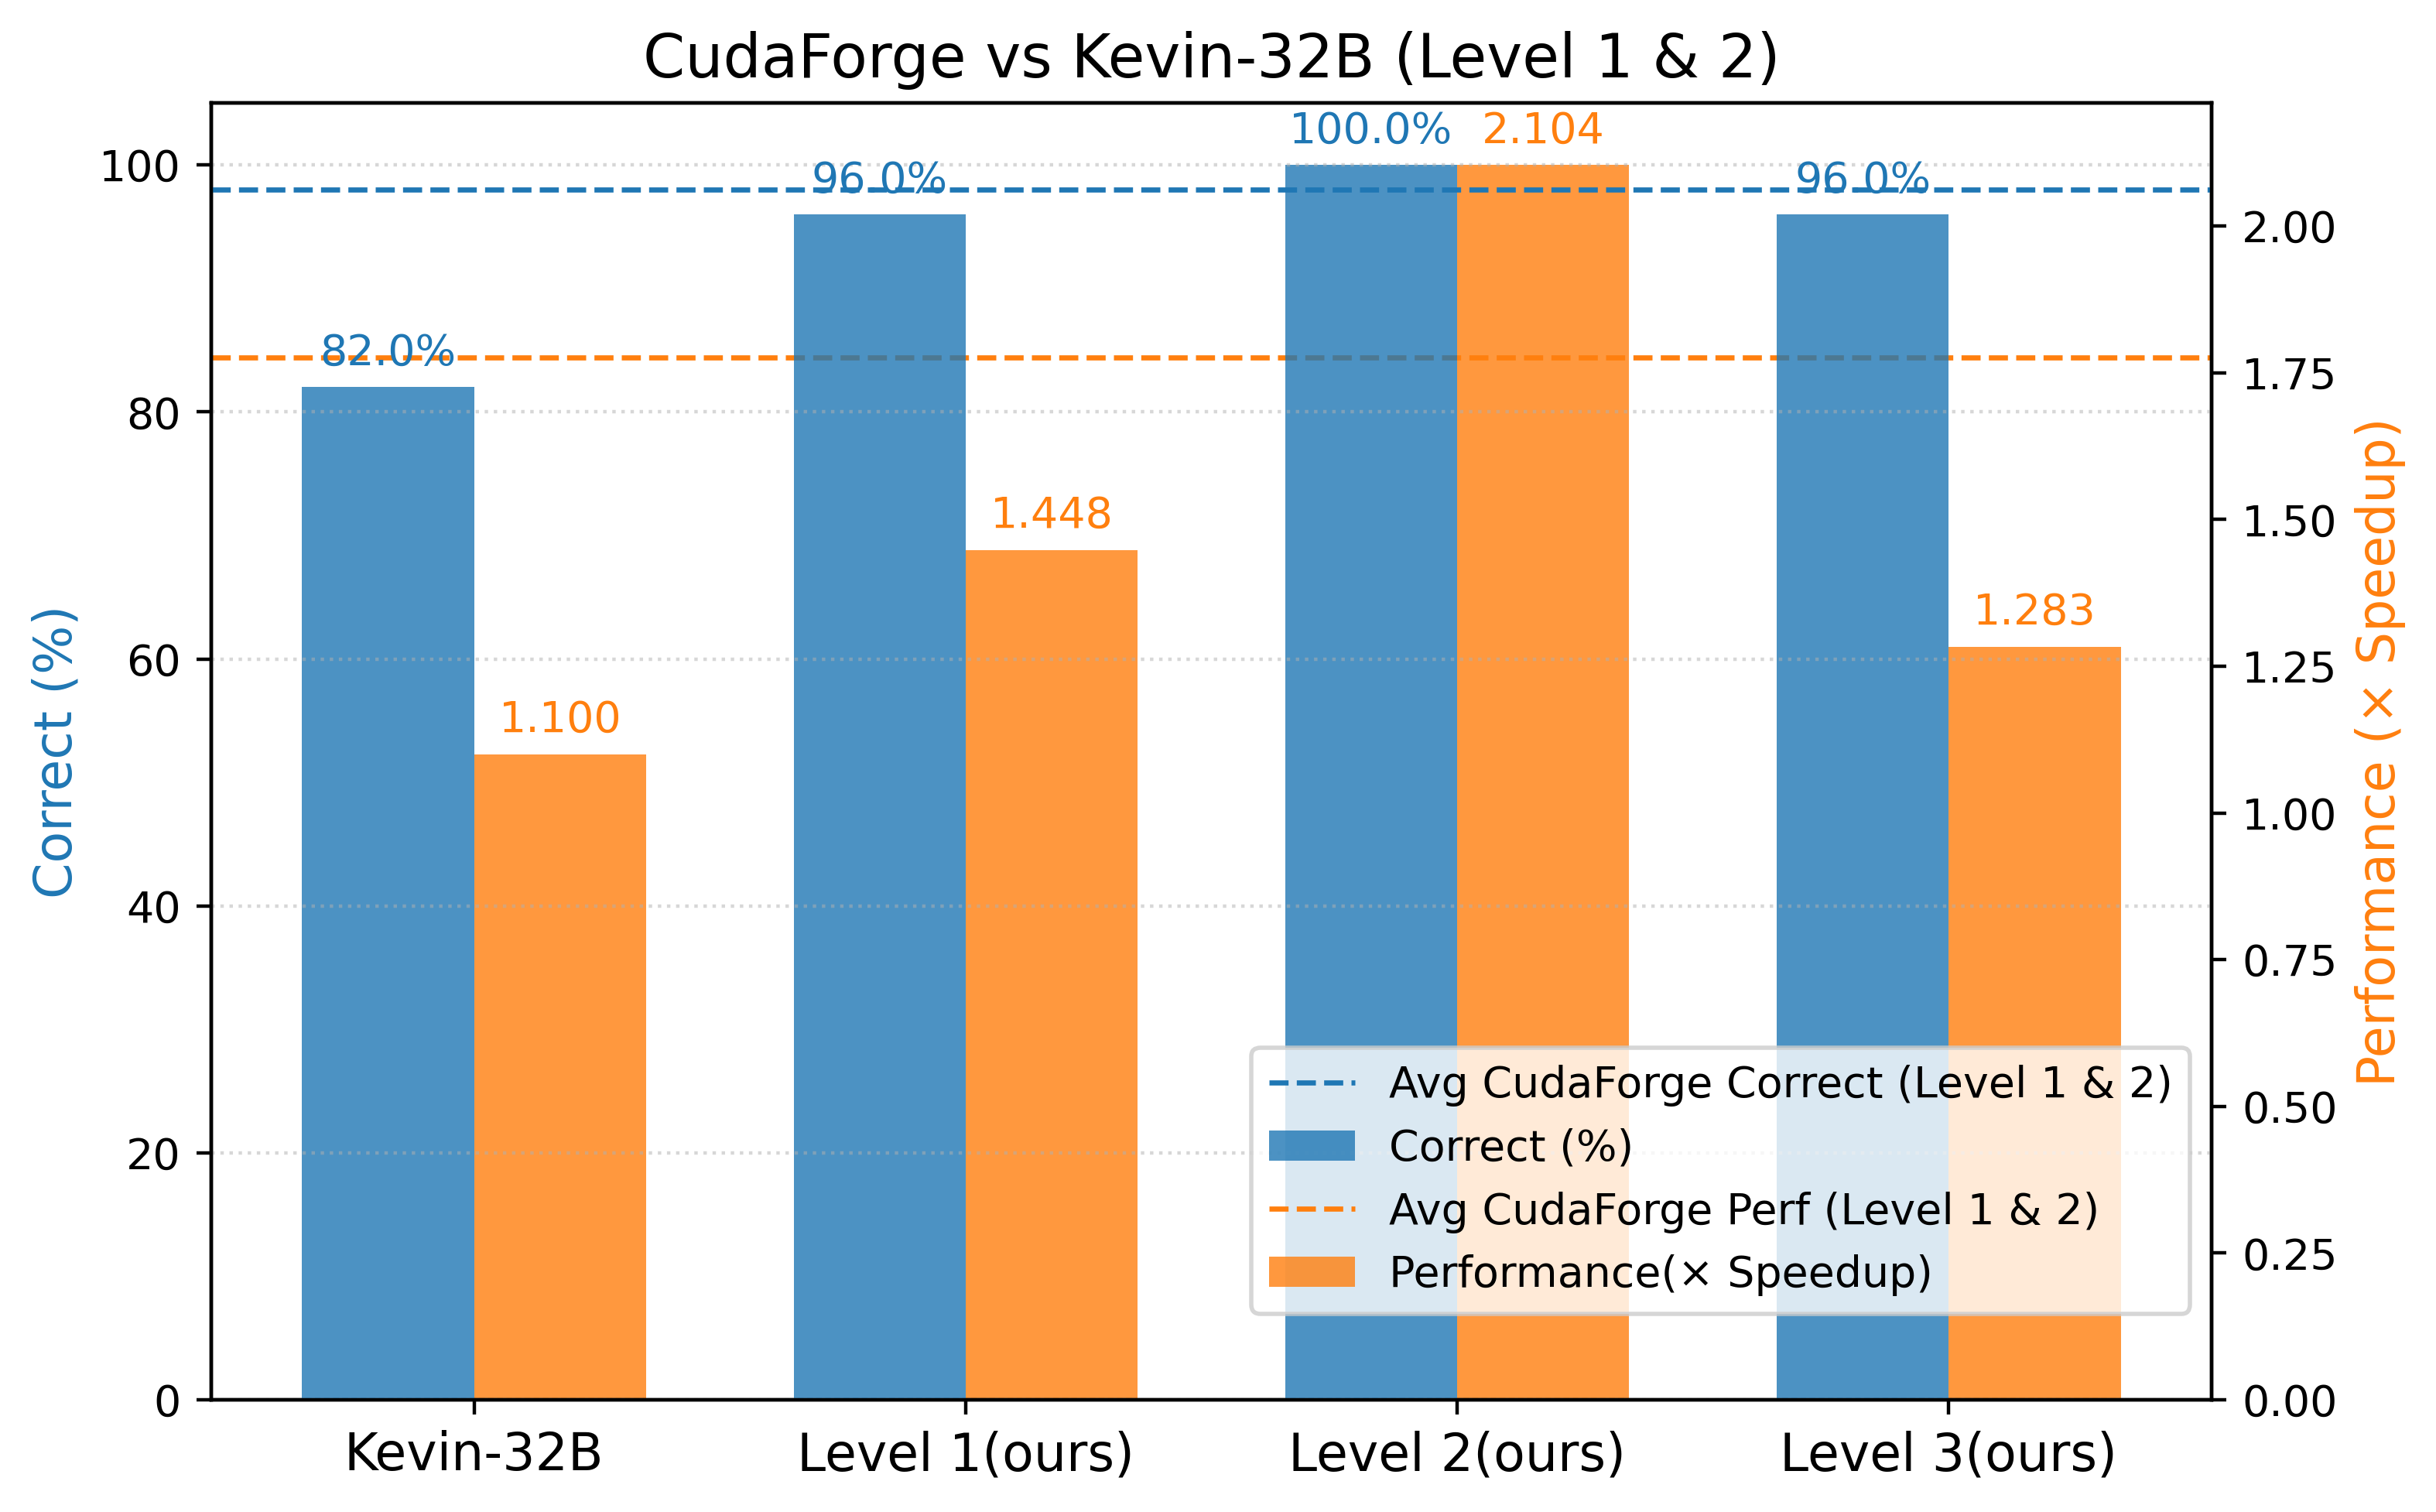
\includegraphics[width=0.85\linewidth]{pic/kevin_benchmark.png}
    \caption{
        Comparison of correctness and performance between \agentname~and Kevin-32B on KernelBench. Dashed lines denote average results of \agentname~over Level 1 and 2. While training-free, \agentname~outperforms Kevin-32B in KernelBench Level 1-2, and gets outstanding results in Level 3.
    }
    \label{fig:kevin}
\end{figure}



As shown in Figure~\ref{fig:kevin}, \agentname~achieves consistently higher correctness and performance across all levels.
In the tasks comparable to Kevin’s benchmark (Levels 1 \& 2), \agentname~reaches an average of \textbf{98.0\%} correctness and \textbf{1.662$\times$} performance, outperforming Kevin-32B’s {82.0\% correctness} and {1.10$\times$ speedup}.
Even in the most challenging Level 3 tasks, \agentname~maintains strong results with \textbf{96.0\%} correctness and \textbf{1.261$\times$} performance, demonstrating its robustness on complex CUDA kernels.

These findings highlight that, despite being a training-free framework, \agentname~surpasses the RL-trained Kevin-32B in both reliability and efficiency.
We attribute this advantage to the effective use of hardware feedback and the design of workflow, which enables \agentname~to perform targeted hardware-aware optimizations rather than rely solely on (potentially inefficient) RL training.

\subsection{API and Computation Time Cost of \agentname}
We evaluate both the API and computation time costs of \agentname~on the KernelBench dataset~$\mathcal{D^*}$. 
The {API cost} is measured as the total expenditure per kernel generation task, 
while the {computation time} is measured as the end-to-end wall-clock time, 
including kernel compilation and execution, model generation, and NCU profiling. 
All experiments are conducted on a single RTX~6000 GPU.  

\begin{table}[t]
\caption{
Comparison of API and computation time cost between \agentname~and the Agentic Baseline~\citep{lange2025robustagenticcudakernel}.
}
\label{tab:cost}
\centering
\begin{tabular}{lccccc}
\toprule
\textbf{Method} & \textbf{Metric} & \textbf{Average} & \textbf{Level 1} & \textbf{Level 2} & \textbf{Level 3} \\
\midrule
\multirow{2}{*}{Agentic Baseline} 
 & API Cost (\$) & 5.0 & --- & --- & --- \\
 & Time (min) & 60.0 & --- & --- & --- \\
\midrule
\multirow{2}{*}{\agentname} 
 & API Cost (\$) & \textbf{0.30} & \textbf{0.29} & \textbf{0.30} & \textbf{0.33} \\
 & Time (min) & \textbf{26.5} & \textbf{28.5} & \textbf{24.1} & \textbf{27.1} \\
\bottomrule
\end{tabular}
\vspace{-0.5em}
\end{table}



As shown in Table~\ref{tab:cost}, \agentname~requires on average only {26.5 minutes} of wall-clock time on a single RTX~6000 GPU and incurs merely {\$0.3} of API cost per kernel. 
This is highly cost-efficient compared with the Agentic Baseline~\citep{lange2025robustagenticcudakernel}, 
which reports approximately {6 GPU hours on H100} and {\$5} per kernel in their Appendix~E.  

\begin{figure}[t]
\centering
\begin{subfigure}[t]{0.48\textwidth}
    \centering
    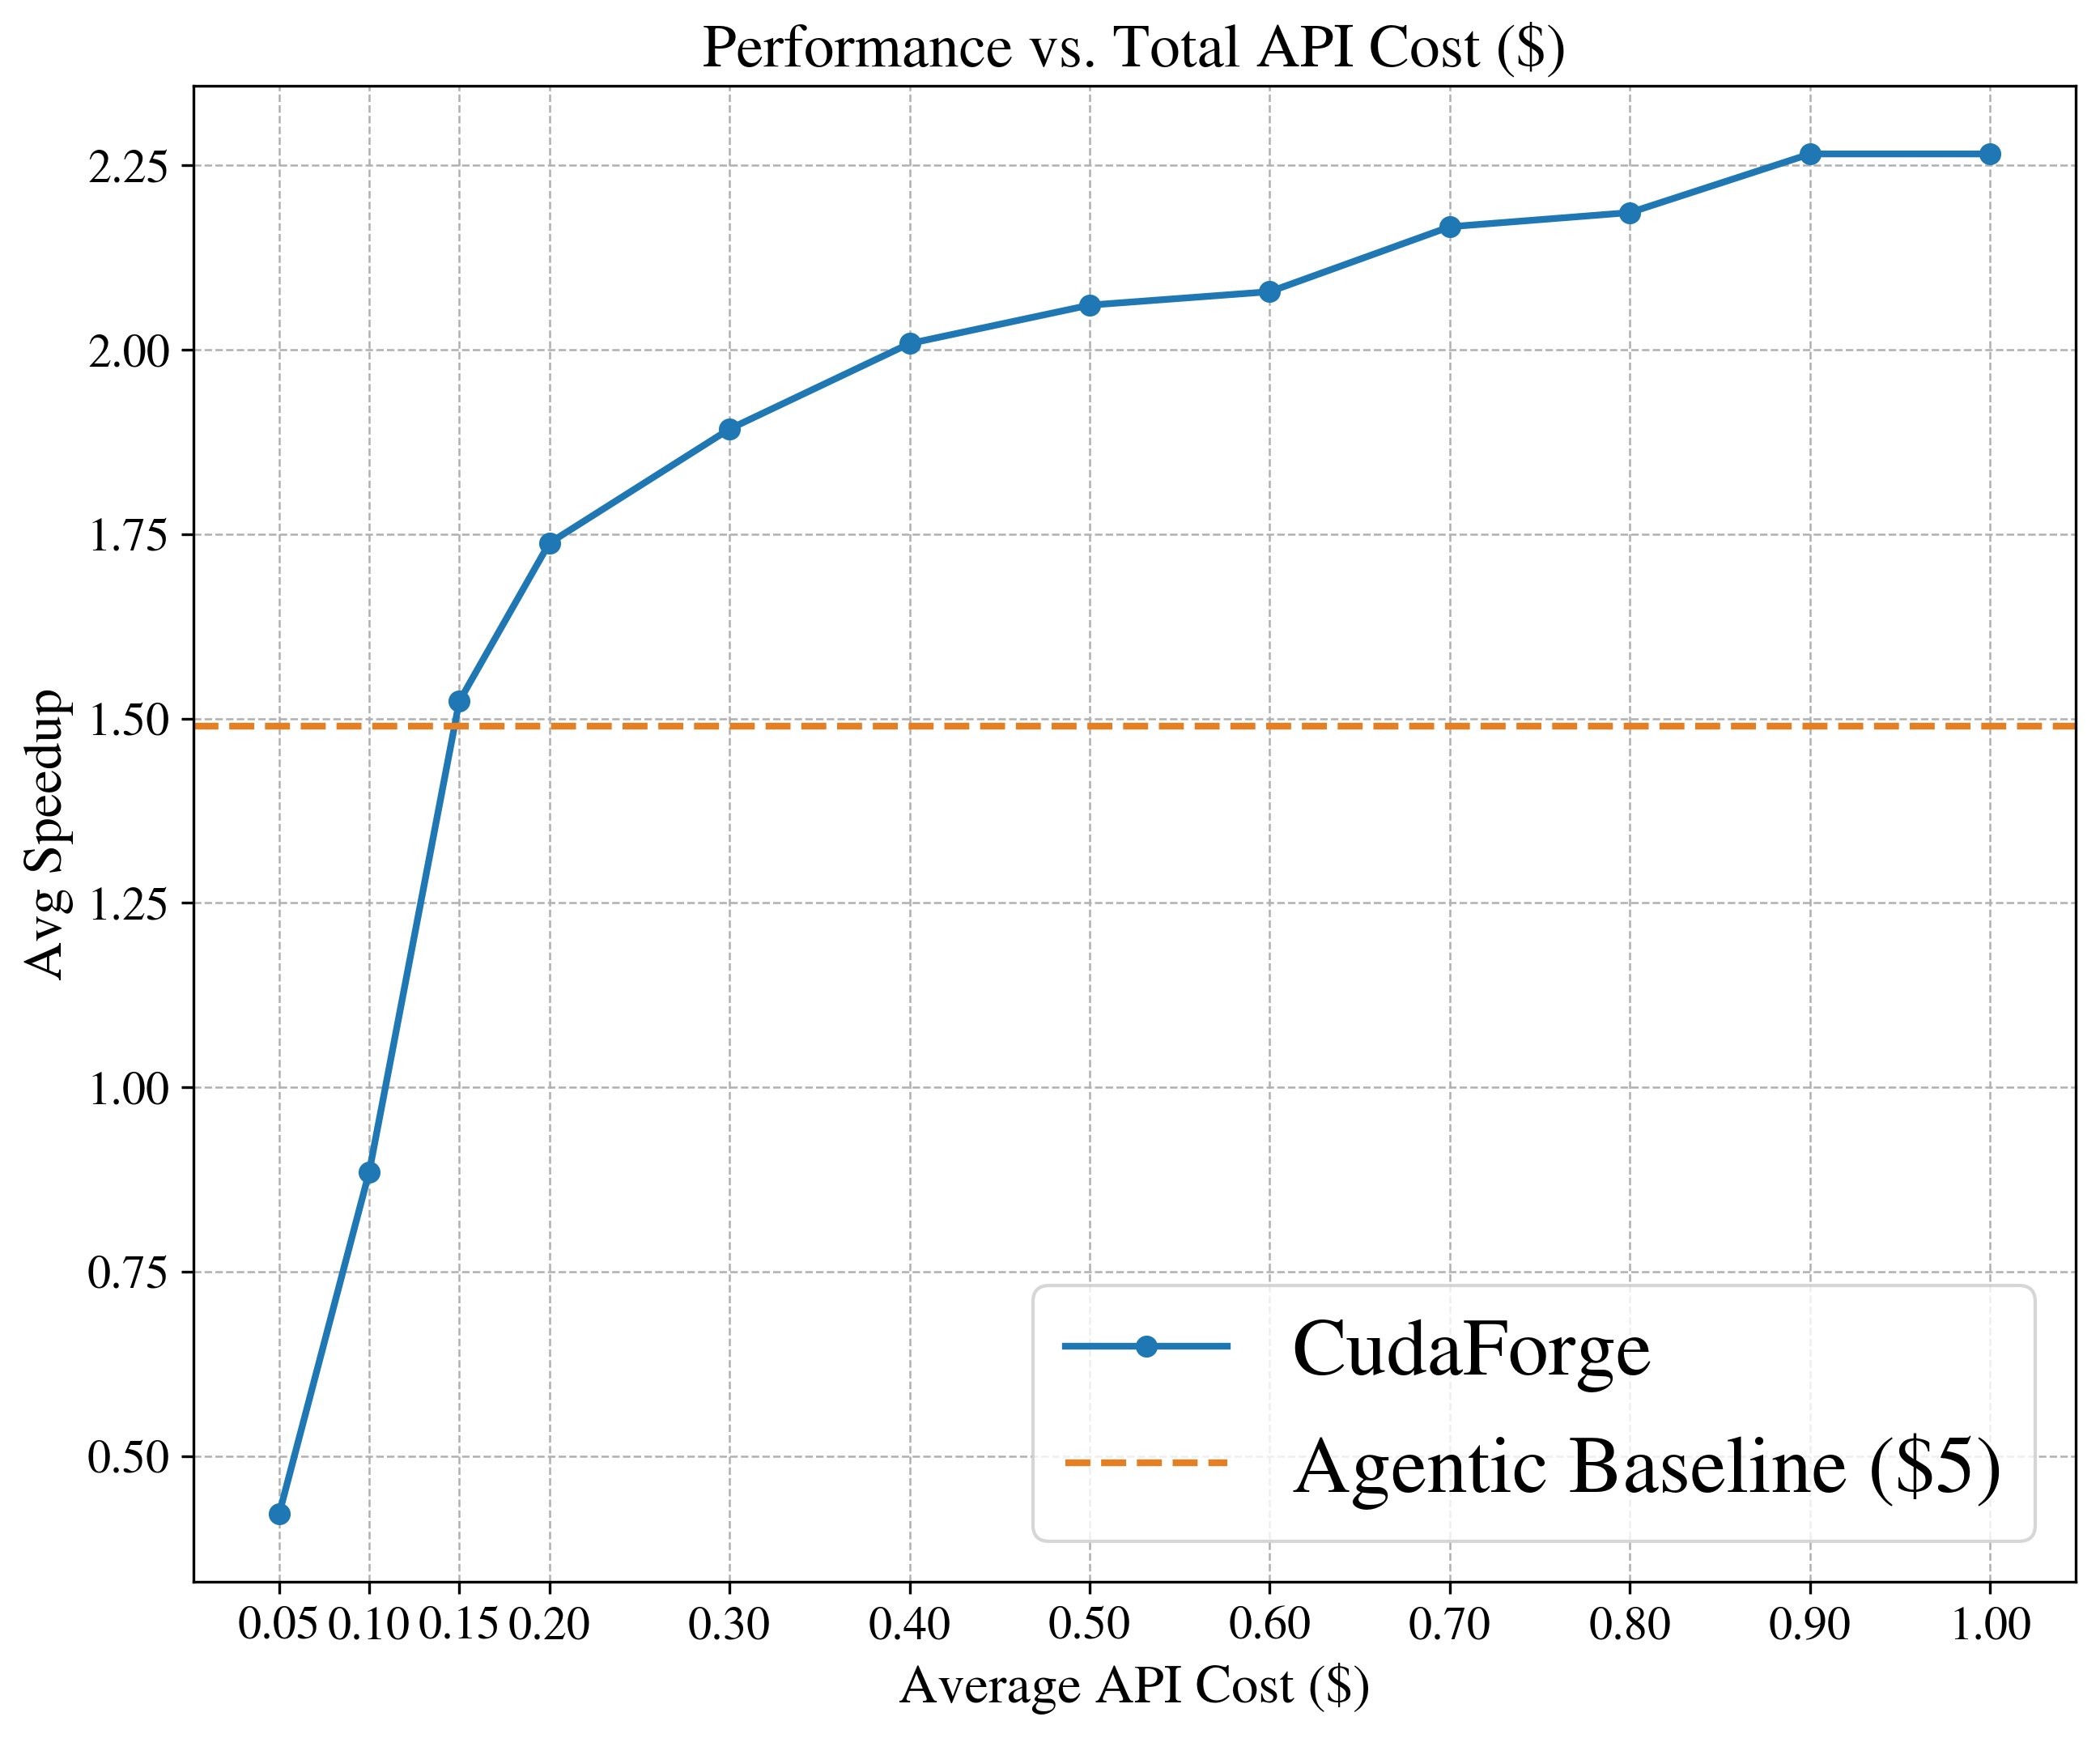
\includegraphics[width=\linewidth]{pic/api.png}
    \caption{Performance vs. API cost of \agentname.}
    \label{fig:api_cost}
\end{subfigure}
\hfill
\begin{subfigure}[t]{0.48\textwidth}
    \centering
    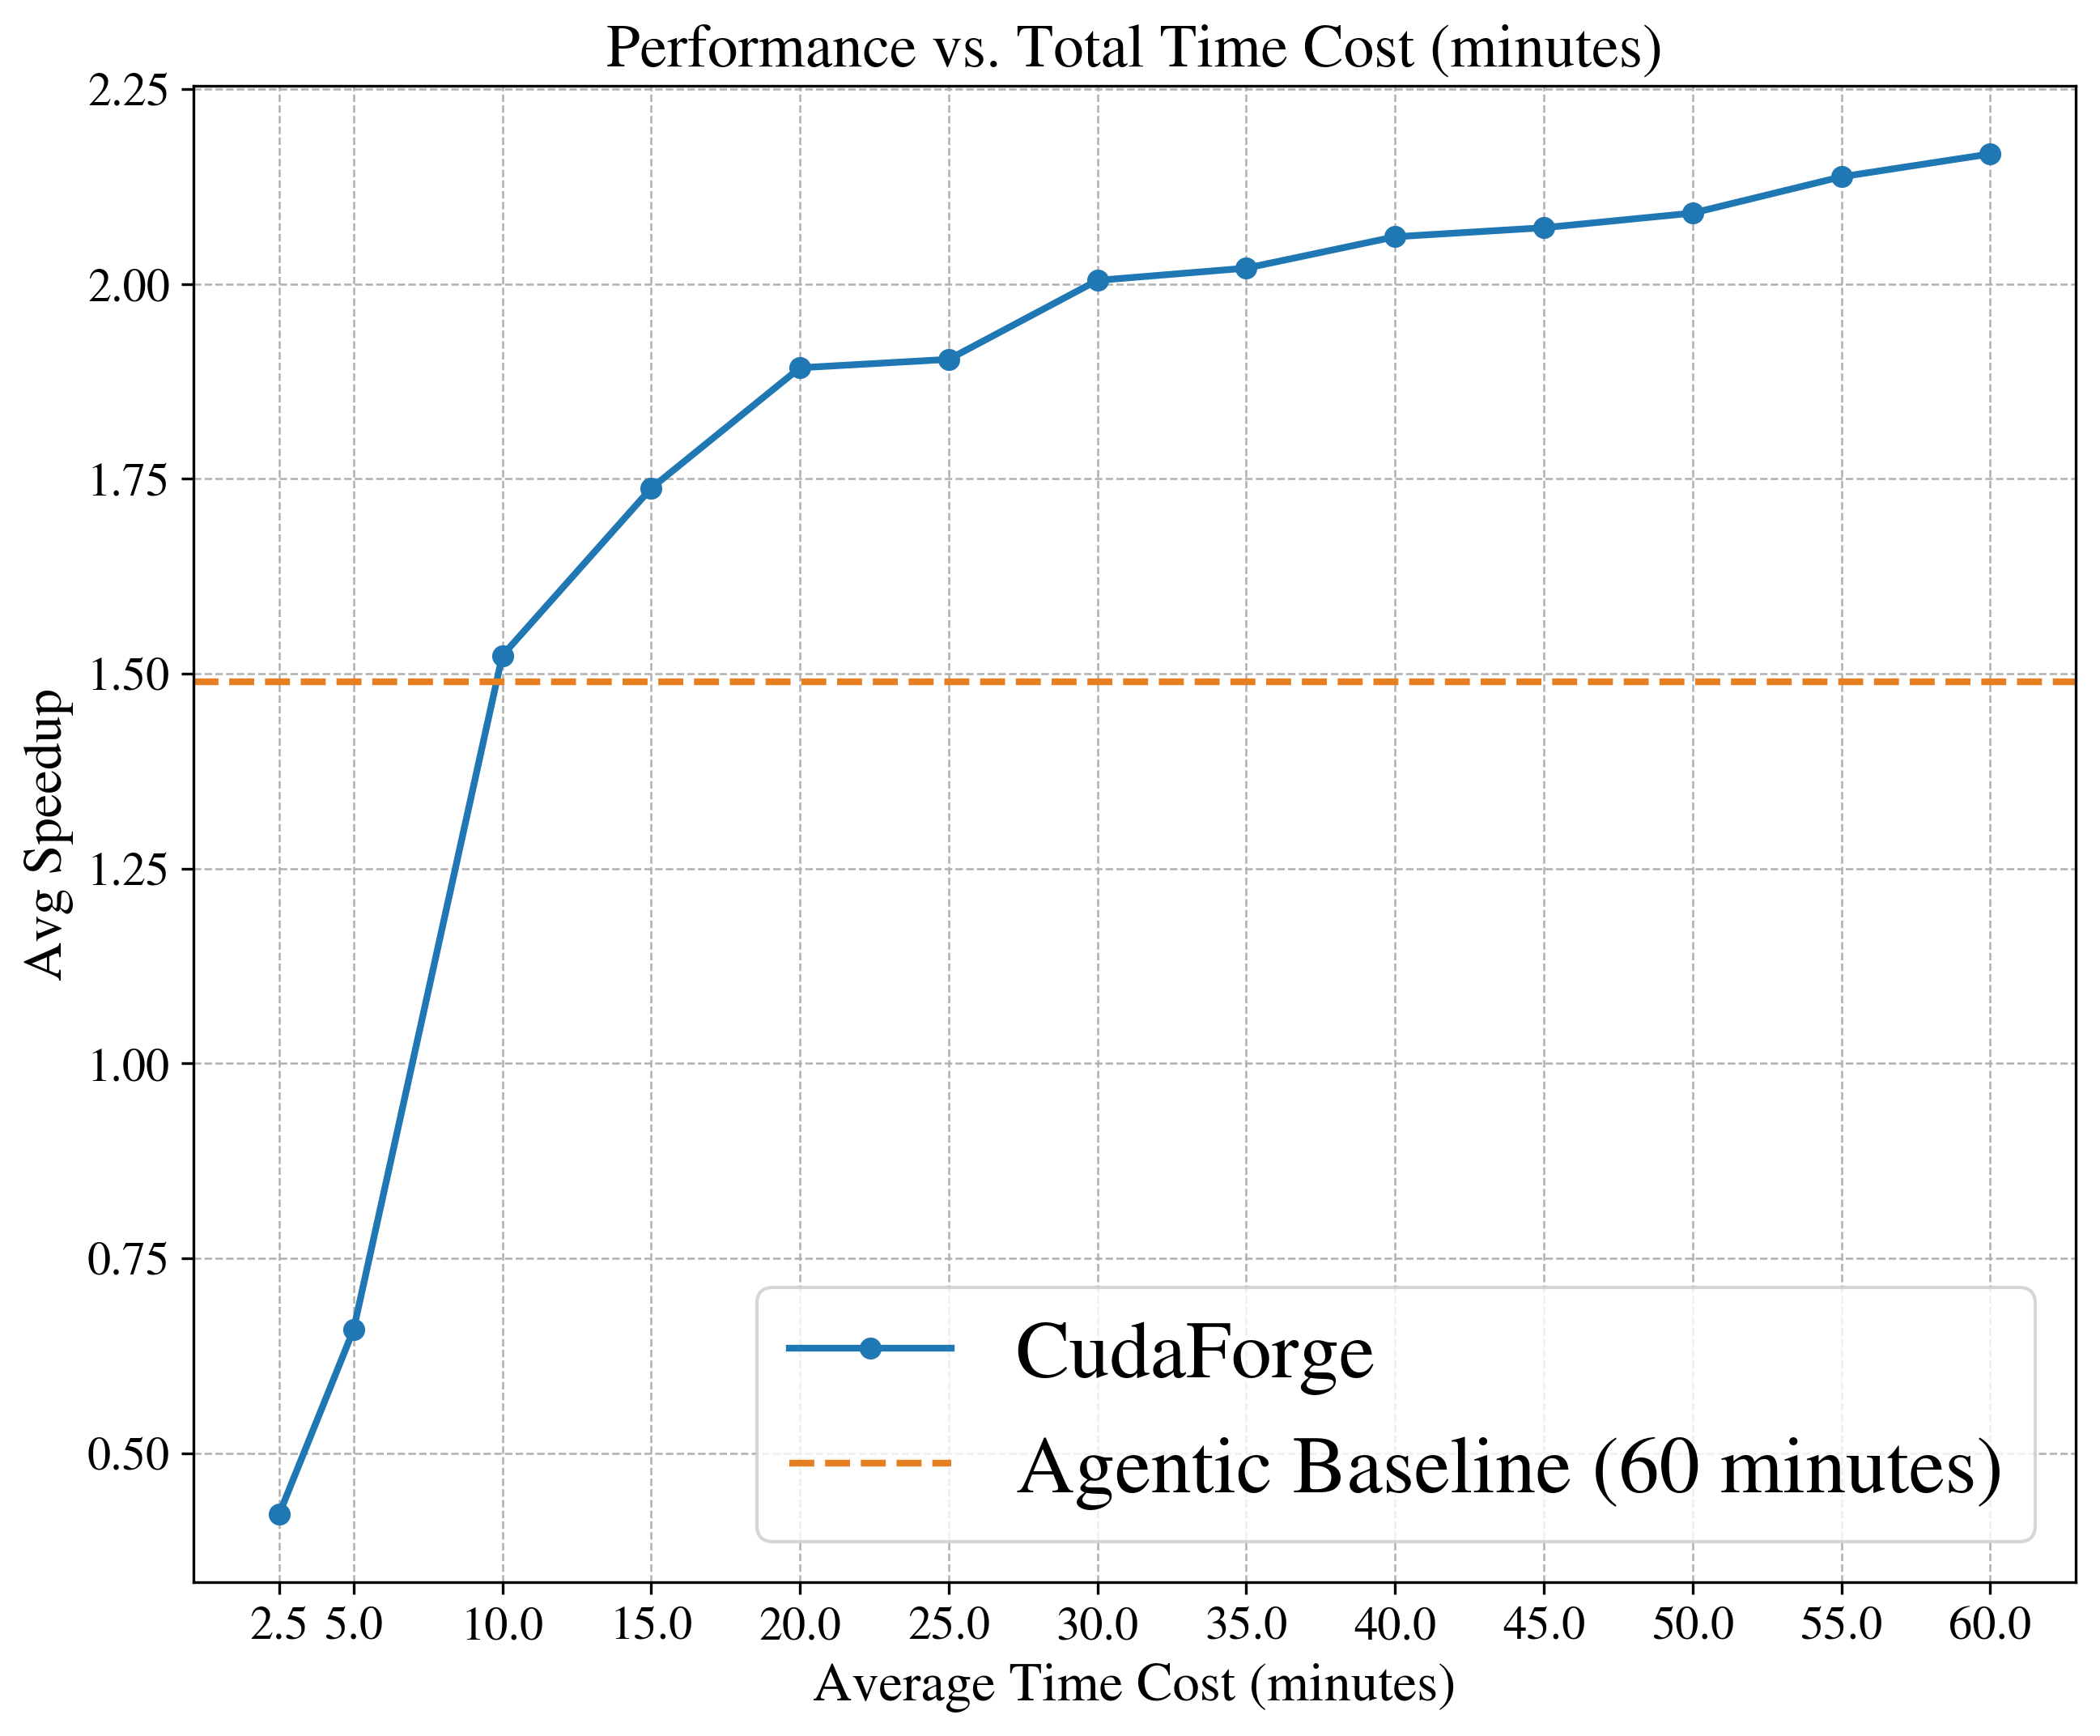
\includegraphics[width=\linewidth]{pic/time.png}
    \caption{Performance vs. computation time of \agentname.}
    \label{fig:time_cost}
\end{subfigure}
\vspace{-0.5em}
\caption{
Relationship between cost and performance of \agentname.
Both API and computation time exhibit a monotonic correlation with performance.
\agentname~already surpasses the Agentic baseline while using no more than {\$0.15} and {10 minutes} per task.
}
\label{fig:apicost_timecost}
\vspace{-0.5em}
\end{figure}

We further analyze how the API and computation costs relate to \agentname's performance, as illustrated in Figure~\ref{fig:api_cost} and~\ref{fig:time_cost}. 
The performance of \agentname~monotonically improves as the API and computation time increase. 
Notably, \agentname~already surpasses the Agentic baseline~\citep{lange2025robustagenticcudakernel} while using no more than {\$0.15} and {10 minutes} per task, 
demonstrating its strong cost–performance tradeoff.

We attribute \agentname's cost efficiency to three main factors:
\begin{enumerate}
    \item \textbf{leveraging hardware feedback.}  
    The Judge leverages hardware feedback to diagnose the current bottleneck and provide targeted, actionable optimization guidance to the Coder. 
    This focused refinement avoids blind exploration and accelerates convergence, thereby reducing the number of API calls and profiling rounds.  

    \item \textbf{Selective NCU metrics.}  
    Instead of profiling the entire metric set, \agentname~uses a curated subset of critical NCU metrics. 
    This not only shortens NCU profiling time but also reduces API cost, as fewer metrics decrease the input token length in Judge queries. 
    \item \textbf{Lightweight memory.}
    In each iteration, both the Coder and Judge are prompted with current round's information, instead of using the full conversation history. 
    This lightweight memory design minimizes redundant context tokens and computation overhead, allowing each agent to focus solely on the most recent feedback and candidate kernel. 
\end{enumerate}




\subsection{Ablation Studies}
\label{ablation}
\paragraph{{Comparison with using the entire set of NCU metrics.}}
\label{NCU}
A key design choice in \agentname~is to filter the full set of NCU metrics and retain only a subset of 24 critical metrics for the Judge.
This selective design allows the Judge to focus on the most informative performance indicators, avoiding redundancy and enabling more consistent optimization feedback.
We conduct an ablation study to evaluate this choice.
As shown in Table~\ref{tab:main_results}, using the complete set of NCU metrics leads to lower correctness and performance, as the Judge is overwhelmed by excessive, partially redundant signals.
Moreover, profiling with all NCU metrics substantially increases inference cost—each kernel requires approximately 40 miuntes on an RTX 6000 GPU and incurs about \$1 in API cost—whereas our selective-metric design achieves superior performance with far lower overhead(26.5 minutes on an RTX 6000 and \$0.3 in API cost).
These results confirm that concise, focused hardware feedback is both more effective and more efficient than exhaustive profiling. We also provide a case study in Appendix~\ref {app:why_subset}.

\paragraph{Comparison with o3-self-refine.}  
A key motivation behind \agentname~is to decouple the roles of generation and evaluation.  
In o3-self-refine, the same model performs ten rounds of self-refinement, implicitly taking on both roles: it must both propose new kernels and evaluate its own outputs based on hardware feedback and runtime signals.  
While this strategy improves the correctness percentage from 57.6\%  to 92.8\%, performance remains limited ({1.107$\times$} speedup, {55.2\% Fast$_1$}).  
In contrast, \agentname~explicitly separates responsibilities: the Coder focuses on code generation, while the Judge specializes in providing structured feedback.  
This division of labor proves critical—allowing each agent to concentrate on a distinct reasoning process—and results in significantly higher efficiency ({1.677$\times$} speedup, {70.8\% Fast$_1$}) without sacrificing correctness.
\label{Ablation-agents}
\paragraph{Comparison with o3-correction (correction-only Judge).}  
In o3-correction, the Judge only provides correction feedback based on runtime signals, without optimization feedback.  
This setting achieves the same {97.6\% correctness} as \agentname, confirming that iterative error correction is sufficient to ensure reliable kernel generation.  
However, efficiency remains much lower, with only {1.222$\times$} performance and {58.8\% Fast$_1$}.  
The contrast with \agentname (\textbf{1.677$\times$}, \textbf{70.8\%}) highlights that while correctness feedback stabilizes generation, performance feedback (grounded in hardware profiling) is essential for driving substantial efficiency gains.

\paragraph{Comparison with o3-optimization (optimization-only Judge).}  
We also evaluate the variant where the Judge provides only optimization feedback, without correction feedback.  
In this setting, the Coder frequently generates kernels that fail to compile or run, since functional errors remain uncorrected.  
As a result, overall correctness is substantially lower than \agentname, and the potential benefits of optimization guidance cannot be realized.  
This outcome demonstrates that correctness feedback is a prerequisite: Without first ensuring functional validity, optimization feedback alone is ineffective and often wasted.  
In contrast, \agentname~leverages both correction and optimization feedback, enabling stable kernel generation and consistent efficiency improvements.


\subsection{Generalization Capability of \agentname}
In this section, we analyze \agentname's capabilities across various maximum iteration num $N$, GPU architectures and base models. Considering the high cost of full experiment, we use the stratified subset \(\mathcal{D}^{*}\) for this section. 


\noindent{\bf Scaling up the maximum number of iteration rounds.}\label{scalingN}
We investigate the effect of the maximum iteration number $N$ on \agentname’s performance. 

\begin{figure}[hbp]
  %\vspace{-4pt}
  \centering
  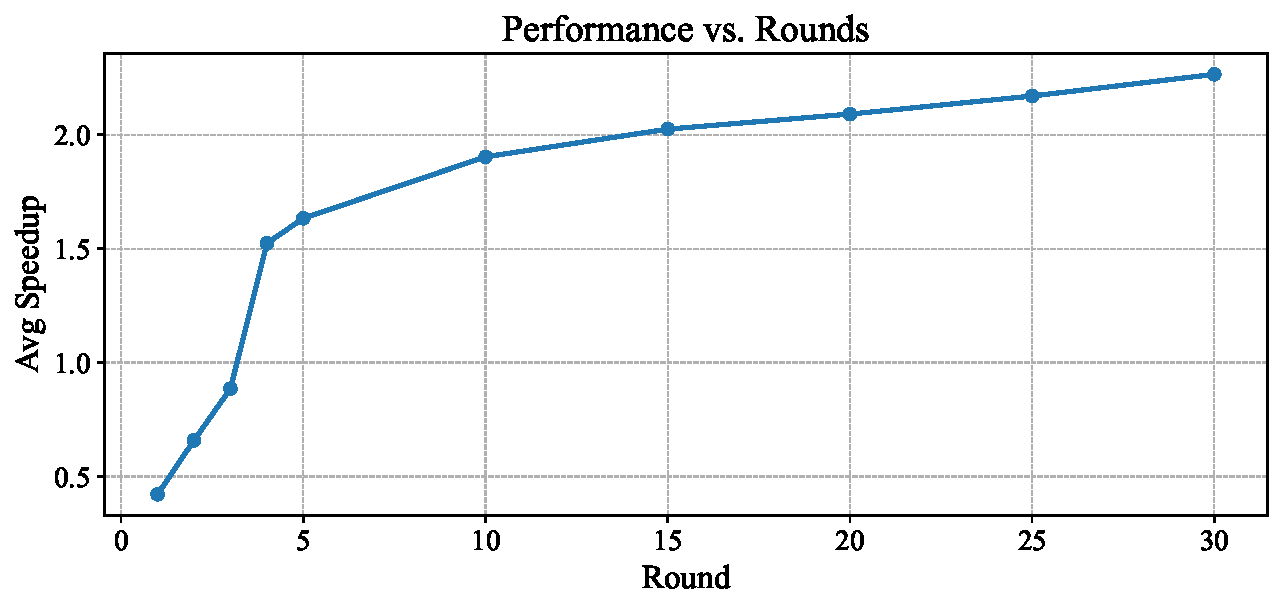
\includegraphics[width=0.6\linewidth]{pic/round_progress_v2.pdf}
  \caption{Scaling the number of iteration rounds to 30 on KernelBench (subset $\mathcal{D}^{*}$).}
  \label{fig:scaling_N}
  %\vspace{-2pt}
\end{figure}

As shown in Figure~\ref{fig:scaling_N}, increasing $N$ from 1 to 10 leads to substantial performance gains, indicating that \agentname~can rapidly improve kernel efficiency through iterative refinement. 
Further increasing $N$ from 10 to 30 continues to improve performance, though with a slower growth rate, suggesting that the system gradually approaches its performance ceiling. After 30 rounds of optimization, \agentname~increases the average speedup to 2.271$\times$.
These results demonstrate that \agentname~benefits from scaling up and has the potential to achieve even stronger performance given larger $N$ with additional inference cost.

\noindent{\bf Using \agentname~in different GPUs.}
\begin{table}[t]
\caption{\agentname's performance on different GPUs. The system consistently achieves high correctness and strong performance across architectures by incorporating GPU specifications and \textit{Nsight Compute} profiling signals during optimization.}
\label{tab:cross_gpu}
\centering
\begin{tabular}{lccccc}
\toprule
\textbf{GPU} & \textbf{Correct$\uparrow$} & \textbf{Median $\uparrow$}  & \textbf{75\% $\uparrow$}  & \textbf{Perf $\uparrow$}  & \textbf{Fast$_1$$\uparrow$} \\
\midrule
RTX 6000(Ada Arch-Data center level)   & 100\% &  1.322 & 1.736 & 1.767 & 84.0\% \\
RTX 4090(Ada Arch-Desktop level)  & 100\% & 1.188 & 1.589 & 1.327 & 80.0\% \\
A100(Ampere Arch-Data center level)  & 100\% & 1.371& 1.762 & 1.841 & 84.0\% \\
RTX 3090(Ampere Arch-Desktop level)  & 100\% & 1.155& 1.706 & 1.320 & 72.0\% \\
\bottomrule
\end{tabular}
\end{table}
We also evaluate \agentname~ on various GPU architectures, including RTX 6000, RTX 4090, RTX 3090 and A100, to examine its effectiveness under different hardware conditions.  
As shown in Table~\ref{tab:cross_gpu}, \agentname
~consistently achieves high correctness and strong performance on all tested GPUs. This is a direct consequence of its design: during the optimization phase, the Judge explicitly incorporates hardware feedback, including NCU metrics and GPU specifications when generating feedback to Coder. This allows the Coder to produce kernels that are tailored to the target GPU at inference time, without training.

\noindent{\bf Instantiate \agentname~with various LLM.}
\begin{table}[t]
\caption{Performance of \agentname~with different base model combinations. We fix one agent as OpenAI-o3(denoted as O3) and replace the other with various models. All combinations achieve strong results, showing that the framework is not tied to a specific base model.} 
\label{tab:base_models}
\centering
\begin{tabular}{lccccc}
\toprule
\textbf{Models (Coder/Judge)} & \textbf{Correct$\uparrow$} & \textbf{Median $\uparrow$}  & \textbf{75\% $\uparrow$}  & \textbf{Perf $\uparrow$}  & \textbf{Fast$_1$$\uparrow$} \\
\midrule
O3 / O3            & 100\% &  1.322 & 1.736 & 1.767 & 84.0\% \\
\midrule
O3 / GPT-5          & 100\% & 1.131 & 1.561 & 2.114 & 96.0\% \\
O3 / Claude-Sonnet-4         & 100\% & 1.265 & 1.456 & 1.829 & 84.0\% \\
O3 / GPT-OSS-120B    & 100\% & 1.226 & 1.490 & 1.364 & 76.0\% \\
\midrule
GPT-5 / O3           & 100\% & 1.125 & 1.388 & 1.896 & 72.0\% \\
Claude-Sonnet-4 / O3          & 88\% & 1.052 & 1.207 & 1.398 & 56.0\% \\
GPT-OSS-120B / O3    & 96\% & 1.080 & 1.477 & 1.653 & 68.0\% \\
QwQ / O3   & 84\% & 0.965 & 1.153  & 0.790 & 44.0\% \\
\bottomrule
\end{tabular}
\end{table}
To examine whether \agentname~depends on a specific base model, we conduct experiments by fixing one side (Coder or Judge) as \textit{OpenAI-o3}(denoted as O3) and replacing the other with various advanced LLMs, including \textit{QwQ-32B}, \textit{GPT-5}, \textit{Claude-Sonnet-4}, and \textit{GPT-OSS-120B}.  
As shown in Table~\ref{tab:base_models}, all combinations achieve high correctness and strong performance, comparable to or even surpassing the original O3/O3 configuration.  
These results indicate that \agentname~is not tied to a specific base model: its effectiveness stems from the workflow of Coder and Judge, and it can readily benefit from stronger models as they emerge.
